%%%%%%%%%%%%%%%%%%%%%%%%%%%%%%%%%%%%%%%%%%%%%%%%%%%%%%%%%%%%%%%%%%%%%%%%%%%%
%% Trim Size: 9.75in x 6.5in
%% Text Area: 8in (include Runningheads) x 5in
%% ws-ijait.tex   :   01-10-2014
%% Tex file to use with ws-ijait.cls written in Latex2E.
%% The content, structure, format and layout of this style file is the
%% property of World Scientific Publishing Co. Pte. Ltd.
%%%%%%%%%%%%%%%%%%%%%%%%%%%%%%%%%%%%%%%%%%%%%%%%%%%%%%%%%%%%%%%%%%%%%%%%%%%%
%%

\documentclass{ws-ijait}
\usepackage[super]{cite}
\usepackage{amsmath}

\begin{document}

\markboth{Rahmat et al.}
{Usage of physical and chemical parameter for predicting water quality of Lake Toba using extreme learning machine}

%%%%%%%%%%%%%%%%%%%%% Publisher's Area please ignore %%%%%%%%%%%%%%%
%
\catchline{}{}{}{}{}
%
%%%%%%%%%%%%%%%%%%%%%%%%%%%%%%%%%%%%%%%%%%%%%%%%%%%%%%%%%%%%%%%%%%%%

\title{Usage of physical and chemical parameter for predicting water quality of Lake Toba using extreme learning machine}

\author{Romi Fadillah Rahmat, Eric Suwarno, Mohammad Fadly Syahputra, Maya Silvi Lydia}

\address{Department of Information Technology, University of Sumatera Utara, Alumni Road no. 3\\
Medan, North Sumatera,
Indonesia\\
romi.fadillah@usu.ac.id, 121402071.es@gmail.com, ncha.fadly@usu.ac.id, maya2@usu.ac.id}


\maketitle

\begin{history}
\received{(Day Month Year)}
\revised{(Day Month Year)}
\accepted{(Day Month Year)}
%\comby{(xxxxxxxxxx)}
\end{history}

\begin{abstract}
Lake Toba serves as an important tourism attraction in Indonesia, especially in the region North Sumatera. The development of tourism in Lake Toba increases the concern of environmental issues, especially the water quality. Meanwhile, extreme learning machine (ELM) is a set of neural networks, which has the advantage in the calculation speed. In this paper, we implemented ELM to process water quality data and predict the water quality in Lake Toba. The prediction process is done through the combination of Python and MATLAB environment. Various activation functions is applied to the network to compare the root mean square error rate. The research shows that different activation functions and number of hidden neurons will affect the accuracy of the prediction process.
\end{abstract}

\keywords{extreme learning machines (ELM); water quality; Lake Toba; artificial neural networks.}

\section{Introduction}	

Water in Lake Toba is classified as water resource in polluted condition, especially in Haranggaol Horison subdistrict of Simalungun Regency in North Sumatera province\cite{1}. The waste produced from households, industries, agricultural industries, and public transportations, are the main source of water pollution in Lake Toba. The population of water hyacinth, and the waste from river streams flowing into Lake Toba, are also the source of water pollution in Lake Toba.

While the tourism industry develops in North Sumatera, mainly in Lake Toba, the possibility of environmental issues which occured in Lake Toba, mainly the water quality, is increased. The change of water quality will also affect the water ecosystem in Lake Toba. Therefore, water quality assessment is required in order to control water quality in lake Toba.

Various method has been implemented to process water quality data. Artificial neural network, which has the same working mechanism with the biological brain, has been implemented in several researches, including screw insertion process\cite{2}, electric system stability monitoring\cite{3}, and wind turbine\cite{4}.

The main problem of prediction process using artificial neural network is the computation time, especially when the network receives big amount of data. Shibata \& Ikeda\cite{5} found that the number of hidden neurons used in the artificial neural network correlates with the learning speed of the network itself. Deng \textit{et al.}\cite{6} found that the backpropagation learning algorithm, which is introduced by Werbos\cite{7} and Rumelhart \textit{et al.}\cite{8}, has difficulty in processing data with the big size, which results in slower performance.

Researches have been done in improving the learning speed of the artificial neural network. Chandra \& Sharma introduce parameterized multilayer perceptron\cite{9} and parameterized deep neural network \cite{10} to improve computational time of the artificial neural network. Hinton \& Teh\cite{11} develop the improved deep belief neural networks, resulting in faster learning speed.

Extreme learning machines (ELM) is one of the methods used to improve computational time in artificial neural network. ELM is proposed by Huang \textit{et al.}\cite{12} ELM is introduced to single hidden layer feedforward neural networks, by randomizing hidden layer neurons using Moore-Penrose inverse. This method results in the improvement of computational time.

Extreme learning machine has been implemented in various researches. Fu \textit{et al.}\cite{13} implemented extreme learning machine for liver tumor detection, by examining liver CT scan imagery. Pangaribuan \& Suharjito\cite{14} implemented extreme learning machine for diabetes mellitus diagnosis. Meanwhile, Zhai \& Du\cite{15} implemented extreme learning machine for vegetation species recognition.

In this research, the water quality data is processed using extreme learning machine. The water quality data is obtained from the research done by Rahmat \textit{et al.}\cite{16}, and will be processed by the extreme learning machine. The result of this process will be compared according to the activation function used in the network.

\section{Theoretical Background}

In this research, artificial neural network is applied with extreme learning machine, to increase the speed of prediction process. The theoretical background of the methodology used in this research is explained as follows:

\subsection{Artificial neural networks}

Hammerstrom\cite{17} defines artificial neural networks as a computational structure, which is developed in line with the working mechanism of the biological brain. According to Uhrig\cite{18}, the artificial neural network consists of a set of processing elements, which are joined by the connection of input weights. The processing elements are arranged into the sequence of layers, most commonly classified as input layer, hidden layer, and output layer. Each processing unit receives input from the connection, which will be calculated by the activation function of the unit itself. The result of the activation function will be passed to the other unit.

The two main operations performed by the artificial neural network is training and testing operation [18]. Training a neural network is needed once the architecture of the network has been constructed [19]. Meanwhile, the testing process is performed after training process is done.

Training process is the process where the neural network constructed for the application is given the random input weights. According to \cite{20}, the training process of the artificial neural network is classified to two methods, namely supervised training and unsupervised training. Supervised training is done to the artificial neural network by giving the network sample data with targeted result. Meanwhile, to perform unsupervised training on an artificial neural network, a sample data is processed by the network, without a finite final result.

\subsection{Extreme learning machine (ELM)}
According to Sun \textit{et al.} [21], extreme learning machines (ELM) refers to a learning method applied in artificial neural networks. The architecture of neural network utilized in extreme learning machine is single hidden layer feedforward neural networks.

Extreme learning machines is proposed by Huang \textit{et al.}\cite{12} to increase the calculation speed of artificial neural networks, by randomizing the hidden layer. They stated that the feedforward neural network utilizes slow gradient based learning, which results in longer computational time. The randomization of the hidden layer results in faster computational speed, along with higher processing result accuracy.

A single hidden layer feedforward neural network is defined by \eqref{Eq. 1}:

\begin{equation}
f_{n} (x) = \sum_{i=1}^{n} G_{i} (x, a_{i}, b_{i}) * \beta_{i}, a_{i} \in R^d, b_{i}, \beta_{i} \in R\label{Eq. 1}
\end{equation}

where $G_{i}(\cdot)$ refers to the activation function calculated in the ith hidden neuron, $a_{i}$ refers to the input weight received by the ith hidden neuron from input neuron, $b_{i}$ refers to the bias weight of the hidden neuron, and $\beta_{i}$ refers to output weight of the hidden neuron.

For each additional nodes, $G_{i}$ is defined from the additional node activation function $g$, as described by \eqref{Eq. 2}:

\begin{equation}
G_{i} (x, a_{i}, b_{i}) * \beta_{i} = g(a_{i} \times x + b_{i})\label{Eq. 2}
\end{equation}

Equation \eqref{Eq. 3} is implemented when the hidden neuron implements RBF as the activation function.

\begin{equation}
G_{i}(x, a_{i}, b_{i}) * \beta_{i} = g(b_{i}\parallel x - a_{i} \parallel)\label{Eq. 3}
\end{equation}

Suppose a training data set $ N = \{(x_{i},t_{i}) \mid x_{i} \in R_{n}, t_{i} \in R_{m}, i = 1, ..., L\}$, with $x_{i}$ represents the training data, $t_{i}$ represents the class label of the sample for each instance, and $L$ is defined as the number of hidden nodes. When implementing the extreme learning machine for training the neural network, the steps are done as follows:

\begin{itemlist}
\item Assign input weights $w_{i}$ and biases $b_{i}$, where $i = 1, ..., L$,
\item Calculate the hidden layer output matrix as H,
\item Calculate the output weight, as defined in \eqref{Eq. 4}:
\begin{equation}
\beta = H^\dagger T\label{Eq. 4}
\end{equation}
where $T = [t_{1},...,t_{N}]^T$ and $H^\dagger$ refers to the Moore-Penrose inverse of matrix $H$.
\end{itemlist}

\section{Methodology}

This section provides explanation about the methodology used in the research, including the water quality data utilized in the research.

\subsection{Utilized Data}

This research utilizes water quality data obtained by Rahmat et al.\cite{16}. The water quality data includes physical and chemical parameters recorded in subsequent time. The data is obtained in different locations, as shown in .

\begin{figure}[th]
\centerline{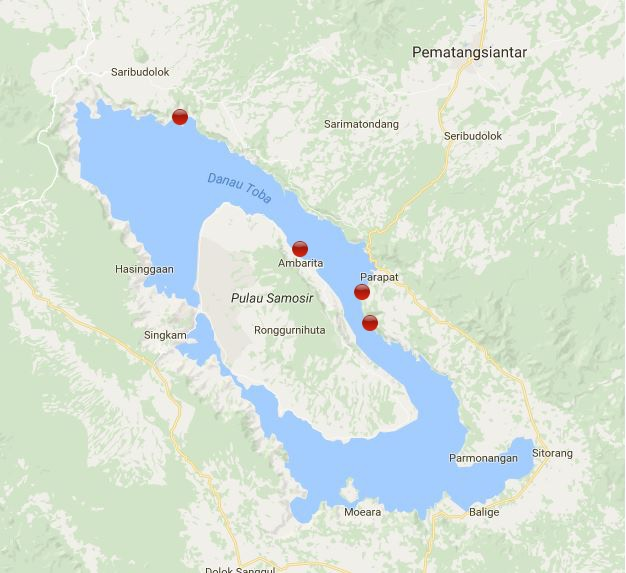
\includegraphics[width=5cm]{map_data_acquisition.jpg}}
\vspace*{8pt}
\caption{Locations of Data Acquisition\cite{16}}
\label{Fig. 1}
\end{figure}

\subsection{General Architecture}

The general architecture of the application is shown by Fig. 2. The development of the application is done in combination of Python and MATLAB environment.

\begin{figure}[th]
\centerline{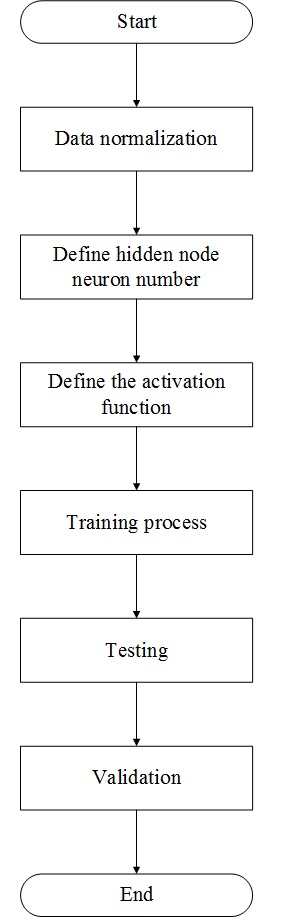
\includegraphics[height=8cm]{general_architecture.jpg}}
\vspace*{8pt}
\caption{General Architecture of the Application}
\label{Fig. 2}
\end{figure}

The general architecture of the application consists of six steps, which are explained as follows:

\begin{enumerate}

\item Data normalization: The water quality data is recorded by Rahmat {\it et al.}\cite{16} by the format shown by Fig 3. The recorded values are separated by semicolon sign, thus needs rearrangement and normalization. According to Patro {\it et al.}\cite{22} , normalization is a pre-processing stage of the problem sets, by which the data will be scaled by the certain range, in order to enable the algorithm to work.

\item Define the number of hidden neuron: This process will be performed after data normalization process is done. According to Heaton\cite{23} , the number of hidden neuron has to be defined by using following rules:

\begin{itemize}
\item the number of hidden neuron ranges from the number of input neuron and the number of output neuron,
\item the number of hidden neuron can be defined as two thirds of the total input and output neuron, and
\item the number of hidden neuron is not higher than twice the number of input neuron
\end{itemize}

Various amount of hidden neuron will be implemented in this research for comparation of the prediction result. The number of hidden neuron varies from 1 to 20.

\item Define the activation function: Dorst\cite{24} defines the activation function is the function implemented in the neuron to determine the state of the neuron in an artificial neural network. In this research, three activation functions will be implemented, respectively sigmoid, sine, and hardlim function, whose result will be compared.

\item Training process: The training process is a process performed in artificial neural network implementation. The training process is performed by using extreme learning machine in the following steps:

\begin{itemlist}
\item Initialize the hidden layer matrix H, consisting of input weights and neuron biases;
\item Calculate the hidden layer output from matrix H;
\item Calculate output weight matrix , which is done according to (4).
\end{itemlist}

\item Testing process: The testing process is performed after the training process is done. The testing process is performed to obtain the result of training process.

\item Validation process: The validation process is performed after the testing process is done. The validation process is performed to verify that the result generated in testing process conforms with the water quality index standard.

\end{enumerate}

The output of the methodology in this research is a graph representing the result of prediction process by the extreme learning machine, followed by the root mean square error of the result.

\section{Experiment and Results}

The process of water quality prediction is done through combination of Python and MATLAB environment. The data normalization process is done through Python environment, while the water quality prediction process is performed through MATLAB environment.

\subsection{Data Normalization}

\begin{figure}
\centerline{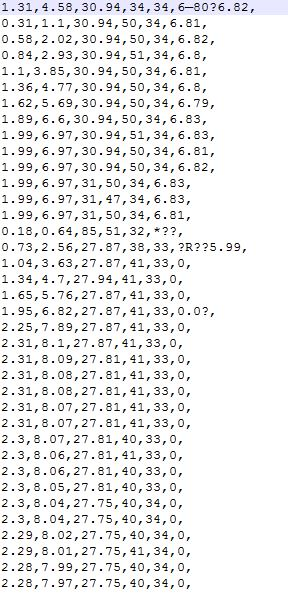
\includegraphics[scale=0.3]{fig-3.jpg}}
\caption{Initial Data Structure\cite{16}}\label{Fig. 3}
\end{figure}

The data normalization process is done through Python environment. The data acquired by Rahmat et al.\cite{16} has the structure shown in Fig 3. The initial data structure is not suitable to be processed with extreme learning machine, thus requiring normalization process.

Before the data is normalized, the initial dataset have to be filtered by each row, to ensure that the value of the recorded data is a valid numeric data. The result of the filtering process is a new dataset with valid numeric value.

The normalization process is performed by using min-max normalization\cite{22}, thus resulting in a dataset with value ranging from -1 to 1, according to \eqref{Eq. 5}:

\begin{equation}
A' = \frac{A - A_{min}}{A_{max} - A_{min}} * (D - C) + C\label{Eq. 5}
\end{equation}

where $A'$ refers to the normalized data value of $A$, with the result ranging from $\mathbb{C}_{D}$. The result of the normalization process will be used by the extreme learning machine regression engine\cite{25}.

\subsection{Water quality prediction}

The water quality prediction process is done through MATLAB environment. The interface of the system is shown in Fig 4.

%figure 4 goes here

To perform the water quality prediction process, the training data and testing data have to be provided to the system. The default architecture of the artificial neural network, which will be constructed after training data is loaded, is SLFN with sigmoid function as the activation function. The hidden layer in 

\section{Conclusion}

The water quality prediction is done by implementing extreme learning machines (ELM), based on the water quality data recorded by Rahmat {\it et al.}\cite{16} , by applying different variations of activation functions and number of hidden neurons.

\begin{thebibliography}{00}

\bibitem{1} D.  Haro, Y.  Djayus and Z.  Harahap, \textquotedblleft Kondisi Kualitas Air Danau Toba di Kecamatan Haranggaol Horison Kabupaten Simalungun Sumatera Utara\textquotedblright , {\it AQUACOASTMARINE}, vol. 1, no. 1, 2013.

\bibitem{2} B. Lara, K. Althoefer and D. Seneviratne, \textquotedblleft Use of artificial neural networks for the monitoring of screw insertions,\textquotedblright \ {\it Proceedings 1999 IEEE/RSJ International Conference on Intelligent Robots and Systems. Human and Environment Friendly Robots with High Intelligence and Emotional Quotients (Cat. No.99CH36289)}, Kyongju, 1999, pp. ~579--584 vol.1.

\bibitem{3} D. Popović, D. Kukolj, and F. Kulić, \textquotedblleft Monitoring and assessment of voltage stability margins using artificial neural networks with a reduced input set,\textquotedblright \ {\it IEE Proceedings - Generation, Transmission and Distribution}, vol. 145, no. 4, p. ~355--362, 1998.

\bibitem{4} R. Ata, \textquotedblleft Artificial neural networks applications in wind energy systems: A review,\textquotedblright \ {\it Renewable and Sustainable Energy Reviews}, vol. 49, pp. ~534-–562, Sep. 2015.

\bibitem{5} K. Shibata and Y. Ikeda, \textquotedblleft Effect of number of hidden neurons on learning in large-scale layered neural networks,\textquotedblright \ in {\it ICCAS-SICE}, Fukuoka: IEEE, 2009, pp. ~5008–-5013.

\bibitem{6} C. Deng, G. Huang, J. Xu, and J. Tang, \textquotedblleft Extreme learning machines: New trends and applications,\textquotedblright \ {\it Science China Information Sciences}, vol. 58, no. 2, pp. ~020301:1–-020301:16, Jan. 2015.

\bibitem{7} P. Werbos. \textquotedblleft Beyond regression: new tools for prediction and analysis in the behavioral sciences,\textquotedblright \ Harvard University, Cambridge, Massachusets, 1974.

\bibitem{8} D. E. Rumelhart, G. E. Hinton, and R. J. Williams, \textquotedblleft Learning representations by back-propagating errors,\textquotedblright \ {\it Nature}, vol. 323, no. 6088, pp. ~533-–536, Oct. 1986.

\bibitem{9} B. Chandra and R. K. Sharma, \textquotedblleft Fast learning for big data applications using parameterized multilayer perceptron,\textquotedblright \ {\it 2014 IEEE International Conference on Big Data (Big Data)}, pp. ~17-–22, 2014.

\bibitem{10} B. Chandra, and R. K. Sharma. \textquotedblleft Fast learning in Deep Neural Networks.\textquotedblright \ {\it Neurocomputing}, vol. 171, pp. ~1205--1215, 2016.

\bibitem{11} G. E. Hinton, S. Osindero, and Y.-W. Teh, \textquotedblleft A fast learning algorithm for deep belief nets,\textquotedblright \ {\it Neural Computation}, vol. 18, no. 7, pp. ~1527-–1554, Jul. 2006.

\bibitem{12} G.-B. Huang, Q.-Y. Zhu, and C.-K. Siew, \textquotedblleft Extreme learning machine: Theory and applications,\textquotedblright \ {\it Neurocomputing}, vol. 70, no. 1-3, pp. ~489-–501, Dec. 2006.

\bibitem{13} F. Huixuan, W. Yuchao and Z. Hongmei, \textquotedblleft Ship rolling motion prediction based on extreme learning machine,\textquotedblright \ {\it2015 34th Chinese Control Conference (CCC)}, Hangzhou, 2015, pp. ~3468--3472.

\bibitem{14} J. J. Pangaribuan and Suharjito, \textquotedblleft Diagnosis of diabetes mellitus using extreme learning machine,\textquotedblright \ {\it 2014 International Conference on Information Technology Systems and Innovation (ICITSI)}, Bandung, 2014, pp. 33-38.

\bibitem{15} C.-M. Zhai and J.-X. Du, \textquotedblleft Applying extreme learning machine to plant species identification,\textquotedblright \ {\it 2008 International Conference on Information and Automation}, Changsha, 2008, pp. ~879--884.

\bibitem{16} R. F. Rahmat, Athmanathan, M. F. Syahputra dan M. S. Lydia, \textquotedblleft Real Time Monitoring System for Water Pollution in Lake Toba,\textquotedblright \ in {\it Proceedings of ICIC 2016}, Lombok, 2016.

\bibitem{17} D. Hammerstrom, \textquotedblleft Neural networks at work,\textquotedblright \ in {\it IEEE Spectrum}, vol. 30, no. 6, pp. ~26--32, June 1993.

\bibitem{18} R. E. Uhrig, \textquotedblleft Introduction to artificial neural networks,\textquotedblright \ {\it Industrial Electronics, Control, and Instrumentation, 1995.}, {\it Proceedings of the 1995 IEEE IECON 21st International Conference on}, Orlando, FL, 1995, pp. ~33--37 vol.1.

\bibitem{19} E. Reingnold and J. Nightingale, \textquotedblleft Training an artificial neural network,\textquotedblright \ in {\it Artificial Neural Networks Technology}, University of Toronto. [Online]. Available: http://www.psych.utoronto.ca/users/reingold/courses/ai/cache/neural3.html. Accessed: Nov. 18, 2016.

\bibitem{20} M. van Heeswijk, \textquotedblleft Advances in extreme learning machines,\textquotedblright \ Aalto University, 2015.

\bibitem{21} M. Gao, W. Xu, H. Fu, M. Wang and X. Liang, \textquotedblleft A Novel Forecasting Method for Large-Scale Sales Prediction Using Extreme Learning Machine,\textquotedblright \ {\it 2014 Seventh International Joint Conference on Computational Sciences and Optimization}, Beijing, 2014, pp. ~602--606.

\bibitem{22} Patro, G. S. Krishna, and K. Kumar, \textquotedblleft Title: Normalization: A Preprocessing stage,\textquotedblright \ 2015. [Online]. Available: http://arxiv.org/abs/1503.06462. Accessed: Jan. 5, 2017.

\bibitem{23} J. Heaton, {\it Introduction to neural networks for Java, 2nd ed}. New York, NY, United States: Heaton Research, United States, 2008.

\bibitem{24} L.Dorst, \textquotedblleft Neural activation functions,\textquotedblright \ in {\it Applications of basic mathematics in Computer Science}. [Online]. Available: https://staff.science.uva.nl/l.dorst/math/sigma.pdf. Accessed: Nov. 22, 2016.

\bibitem{25} Q.-Y. Zhu and G.-B. Huang, \textquotedblleft Extreme learning machines,\textquotedblright \ 2013. [Online]. Available: http://www.ntu.edu.sg/home/egbhuang/elm\textunderscore random\textunderscore hidden\textunderscore nodes.html. Accessed: Jan. 5, 2017.
\end{thebibliography}

\end{document}